\section{Sorting and permutation}

The \emph{sorting} problem gives us an array of values $A[1, n]$ and asks us to sort it with some comparative function.

The \emph{permuting} problem gives us an array of values $A[1, n]$ and a permutation $\Pi[1, n]$ and asks us to implement $\Pi$ over $A$: $A[\Pi[1]], A[\Pi[2]], A[\Pi[3]], A[\Pi[4]]$

Example: $A = [A,B,C,D], \Pi=[3, 1, 2, 4] \implies A_{\Pi} = [C, A, B, D]$

So in the first problem we are looking for the permutation and then we apply it, in the second we are just applying the permutation.
In a paper from 1988 it is proved that in 2-layer model permuting and sorting are equivalent.

\subsection{RAM Model}
In RAM model we already know that sort problem has complexity of $O(nlogn)$ and permuting problem is $O(n)$.

\subsection{2-level Model}
\subsubsection{Naive algorithm}
The naivest algorithm would be:
\begin{verbatim}
    for i = 1, n do
        B[i] = A[PI[i]]
        
    A = B
\end{verbatim}
so it is $\Theta(n)$ in I/O in the worst case since we can access the values of A in sparse order and each time we could hit a non resident block.

\subsubsection{Reduce to sort}
We can otherwise exploit the sorting algorithm to make less memory access:
\begin{verbatim}
    Create couples X = <A[i], i>
    Create couples Y = <PI[i], i> // source, destination

    Sort Y for first element
    Create couples Z = <X[1], Y[2]>

    Sort Z for second element
    
    permutation is Z[1]
\end{verbatim}
The total cost is $3 \cdot O(\frac{n}{B} + 2 \cdot SORT(n)$ so $O(\frac{n}{B} + SORT(n))$

So permuting in 2-level model is actually $O(min\{n, \frac{n}{B} + SORT(n)\})$

\subsubsection{Complexity of sort}
Let's take sort complexity as it is because we will explain it in the future with some reasoning on the algorithms used:
$$
    SORT(n, M, B) = O\left( \frac{n}{B} \cdot log_{\frac{M}{B}} \left( \frac{n}{M} \right) \right) 
$$
Basically we say that we have $\frac{n}{B}$ as the cost of a single scan and $log_{\frac{M}{B}} \frac{n}{M}$ different scans.

Using the logarithm properties of change of base:
$$
    log_{\frac{M}{B}} \frac{n}{M} = \frac{log_2\frac{n}{M}}{log_2 \frac{M}{B}}
$$
So buying more memory the ratio decreases and so we need less runs!

Example: $M=2^{30}$, $B=2^{15}$, $n=2^{60}$:
$$
    \frac{log_2 \frac{2^{60}}{2^{30}}}{log_2 \frac{2^30}{2^15}} = \frac{log_2 2^{30}}{log_2 2^{15}} = \frac{30}{15} = 2
$$
This means that we sort Hexabytes of data in just 3 passes on a machine with 1GB of memory!

Let's call $L=log_{\frac{M}{B}} \frac{n}{M}$:
\begin{itemize}
    \item permute is $O\left(min\{n, \frac{n}{B} \cdot L \}\right)$
    \item sort is $O\left( \frac{n}{B} \cdot L \right)$
\end{itemize}
so it is better to sort than permute when: $\frac{n}{B} \cdot L \leq n \implies B \geq L$

NB: $B$ is $O(30Kb)$ meanwhile $L$ is 2.

\section{Multi-way Mergesort}
\subsection{Binary Mergesort}
The already known binary mergesort sorting approach is based on splitting array in halves, when the partition has size equals to 1 the recursion stops and it starts the merging procedure which produces incrementally large sorted sequences.
Just with that description we can notice that in the case of already sorted array we are doing useless work!

The pseudocode is:
\begin{verbatim}
    Mergesort(A, i, j):
        if(i < j):
            m = floor((i+j)/2)
            Mergesort(A, i, m)
            Mergesort(A, m+1, j)
            Merge(A, i, j, m)
\end{verbatim}

\subsubsection{I/O complexity}
Let's estimate I/O complexity of merge procedure (since the other part of the algorithm is just recursion): let's assume partitions of size $l$ and a block size of $B$.
We load a block from each partition, then those blocks stays in memory until we are done to compute the hole partition which gets replaced with the next one.
So we do:
\begin{itemize}
    \item $\frac{2l}{B}$ I/Os to read the data
    \item $\frac{2l}{B}$ I/O to write back the sorted data
\end{itemize}
so \verb|Merge(A, i, j, m)| is $O\left(\frac{l}{B}\right)$

For each merge the cost is the cost of reading and writing two partitions of the size of that recursion level:
$$
    \frac{l_1 + l_2}{B} + \frac{l_3 + l_4}{B} + ... = \frac{l_1 + l_2 + l_3 + l_4 + ...}{B} = \frac{n}{B}
$$

and we have $log_2 n$ recursive call since we split the array in half at each level, so the total I/O cost is:
$$
    O\left( \frac{n}{B} log_2 n \right)
$$

This analysis is a bit weird since:
\begin{itemize}
    \item $M$ does not appear in the formula
    \item we are not taking into account the fact that in lower recursion level we are working always on the same block until the partition size doesn't get greater than the block size it self cause we don't need to fetch again:
    \begin{figure}[H]
        \centering
        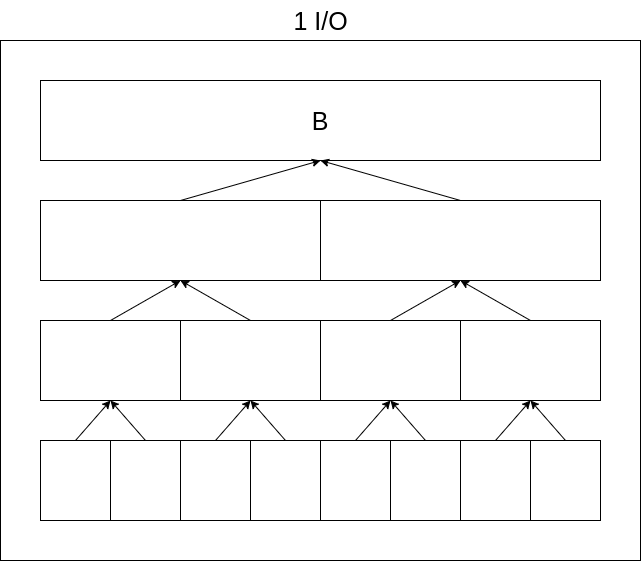
\includegraphics[width=200px]{images/1_Introduction/block_optimization.png}
        \caption{if partition size is less than block size, no new I/O is done}
    \end{figure}
\end{itemize}

So we don't need to fetch blocks at each recursion.
We have: 
\begin{itemize}
    \item $\frac{n}{B}$: cost for all the level with $l <= B$
    \item $\frac{n}{B} \left( log_2 n - log_2 B \right) = \frac{n}{B} log_2 \left( \frac{n}{B} \right)$: cost for all the level with $l > B$
\end{itemize}

The previous argument can be extended to the whole memory instead of the single block: we have no I/O until we reach partition greater than the entire memory.
So the total I/O cost is:
$$
    O\left( \frac{n}{B} log_2 \frac{n}{M} \right)
$$

\subsubsection{Avoid useless recursion}
We can improve the algorithm to avoid some useless recursion: once we are in a partition which fits entirely inside the memory we can avoid other recursion call and insted sort the elements in place with another algorithm, for example heap-sort or quick-sort.

Avoiding useless recursion is nice to have since prevents memory usage avoiding the allocation of new stack frames.

\subsection{Snow Plow}
If we would be able to create longer sorted sequence we could do less recursion and so less scans and I/O operations.

Let's suppose to have $A=[1, 7, 5, 3, 8, 2, 4, 6]$ and $M=3$, we create a set $U$ for the unsorted items and a heap $H$ for the sorted items.
Let's fill the $H$ with $M$ items and keep $U$ empty:
$$ U = [] $$
$$ H = [1, 5, 7] $$
at each iteration we extract the minimum from the heap and insert another item from the array $A$ following the rules:
\begin{itemize}
    \item if the new item is lower than the last extracted item we insert it into $U$;
    \item if the new item is larger or equal than the last extracted item we insert it into $H$
\end{itemize}
Let's do a couple of runs: 
\begin{itemize}
    \item extract 1, insert 3 into $H$:
        $$ U = [] $$
        $$ H = [3, 5, 7] $$
    \item extract 3, insert 8 into $H$:
        $$ U = [] $$
        $$ H = [5, 7, 8] $$
    \item extract 5, insert 2 into $U$:
        $$ U = [2] $$
        $$ H = [7, 8] $$
    \item extract 7, insert 4 into $U$:
        $$ U = [2, 4] $$
        $$ H = [8] $$
    \item extract 8, insert 6 into $U$:
        $$ U = [2, 4, 6] $$
        $$ H = [] $$
\end{itemize}

Once the heap is empty and the unsorted part is full we can terminate our run, so we transfer the elements from $U$ to $H$ and we start again to build the next sorted sequence.

Some pros of this algorithm are:
\begin{itemize}
    \item this algorithm produces sequences of $M$ elements or more;
    \item it's a kind of insertion sort, if the sequence is sorted it just runs in $O(n)$ time
\end{itemize}

Let's estimate on average the length of the produced sequences:
\begin{itemize}
    \item we start from:
        $$ |U| = 0 $$
        $$ |H| = M $$
    \item and we end with:
        $$ |U| = M $$
        $$ |H| = 0 $$
\end{itemize}
Let's suppose that in a run we made $\tau$ reads, so we passed over $M + \tau$ elements, at the end of the run we have:
\begin{itemize}
    \item $\tau$ elements written out;
    \item $M$ elements remain inside $U$
\end{itemize}

To estimate the average we can suppose that on average half of the items will be inserted into $U$, and the other half will be inserted into $H$, so we will have $\frac{\tau}{2}$ elements going into $U$, so we can say that:
$$
    M = \frac{\tau}{2} \implies \tau = 2 \cdot M
$$

So with the snow plow algorithm we are building sequence double the size of the ordinary binary merge-sort!
In that way we are building less taller tree:
$$
    \#levels = log_2 \left( \frac{n}{2M} \right) = log_2 \left( \frac{n}{M} \right) - log_2 2 = log_2 \left( \frac{n}{M} \right) - 1
$$
Only one level less, but we have to recall that each level means a scan and with a lot of data scan means hours of computation!

Example: $A = [1, 8, 3, 2, 5, 0, 6], M = 2$
\begin{itemize}
    \item fill $U$ with $M$ elements:
    $$ U = [1, 8] $$
    $$ H = [] $$
    
    \item build the heap:
    $$ U = [] $$
    $$ H = [1, 8] $$

    \item extract 1, insert 3 in $H$:
    $$ U = [] $$
    $$ H = [3, 8] $$

    \item extract 3, insert 2 into $U$:
    $$ U = [2] $$
    $$ H = [8] $$

    \item extract 8, insert 5 into $U$:
    $$ U = [2, 5] $$
    $$ H = [] $$
    we terminated the first run producing: $[1, 3, 8]$

    \item build the heap:
    $$ U = [] $$
    $$ H = [2, 5] $$

    \item extract 2, insert 0 into $U$:
    $$ U = [0] $$
    $$ H = [5] $$

    \item extract 5, insert 6 into $H$:
    $$ U = [0] $$
    $$ H = [6] $$

    \item extract 6, nothing to insert:
    $$ U = [0] $$
    $$ H = [] $$
    we terminated the second run producing: $[2, 5, 6]$

    \item build the heap:
    $$ U = [] $$
    $$ H = [0] $$
    
    \item extract 0, nothing to insert. We ended the last run producing $[0]$
\end{itemize}
In the end we got 3 sorted sequences: $A = [1, 3, 8, 2, 5, 6, 0]$.

\subsection{Multi-way mergesort}
In terms of number of I/Os how many blocks we fetch for each partition to merge is the same since we are working only on the first blocks of the partitions because the other ones can be used only after the first are merged: 
\begin{figure}[H]
    \centering
    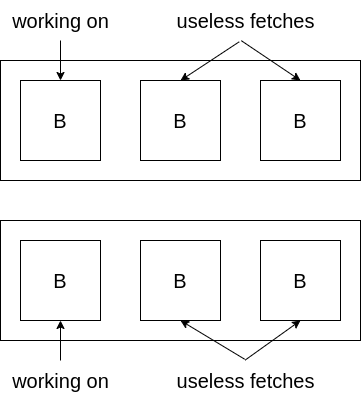
\includegraphics[width=175px]{images/2_Sorting/useless_fetches.png}
    \caption{Useless fetches in binary merge-sort}
\end{figure}

We can exploit that feature to build a k-way merger:
\begin{figure}[H]
    \centering
    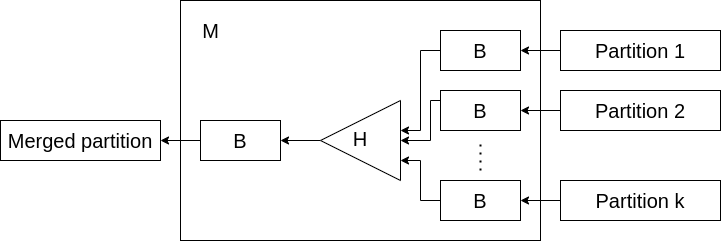
\includegraphics[width=300px]{images/2_Sorting/k-way_merger.png}
    \caption{K-way merger}
\end{figure}
We need to get the minimum among $k$ different values, so we use a min-heap to avoid comparisons, in that way extraction is $O(log_2 k)$ instead of $O(k)$

To refill the heap after one extraction we need to fetch from the same partition the extracted element came from.

Using this algorithm to merge $k$ partition we just need a scan so $O(\frac{n}{B})$.
Merging $k$ sequences at a time is the same as having a recursion tree with $k$ children for each node, so the tree height is $O(log_k \frac{n}{B})$ and so the number of scans to order the array.
In the end the I/O complexity of the algorithm is $O\left( \frac{n}{B}log_k \frac{n}{B} \right)$.

Let's estimate $k$ value: we can merge at most the number of blocks that fits inside the memory, remember that we need another one to build the output partition, so let's suppose that in memory we can have at most $k+1$ blocks:
$$
    (k+1)B \approx M \implies k+1 \approx \frac{M}{B} \implies k \approx \frac{M}{B}-1 \implies k = O \left( \frac{M}{B} \right)
$$

In the end the complexity of sort with $k$-way merge-sort is:
$$
    O\left( \frac{n}{B} log_k \frac{n}{B} \right) = O\left( \frac{n}{B} log_{\frac{M}{B}} \frac{n}{B} \right)
$$

\section{Sort lower bound}
In RAM model we proved that there is a lower bound for sorting problem which is $\Omega(n \cdot log n)$, we proved it using binary decision tree:
\begin{figure}[H]
    \centering
    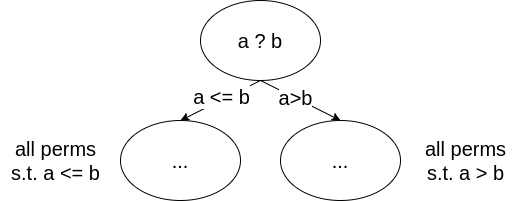
\includegraphics[width=200px]{images/2_Sorting/decision_tree.png}
    \caption{binary decision tree}
\end{figure}
and going down until we reach a node who contains a single partition.
Of course the tree can be unbalanced but the narrowest tree is the balanced one, so the lower bound can be calculated using: $2^t \geq n! \implies t \approx O(n \cdot log n)$.

\subsection{2-layer model}
In this model each node can lead to several comparisons because each node is a fetch and in each block there are various elements that can be fitted in several different places.

Let's count how many ways we have to build the sequence: it's the same problem of asking in which positions will the single elements be placed in the sequence.
That number is the dispositions: $\binom{M}{B}$, so that number is the number of comparison induced by 1 I/O operation.
In this calculation though we have the bias that we know the right permutation of the elements, which is not true, so to count the effective ways we can sort the elements we must also consider the permutations of the single block, but only once, for the first time we see a new block.

We can say:
\begin{itemize}
    \item fetch of new block induces $\binom{M}{B} \cdot B!$ comparisons, let's call it $X$;
    \item fetch of old block induces $\binom{M}{B}$ comparisons, let's call it $Y$
\end{itemize}
so we can build the new tree with both $X$ and $Y$ type nodes.
We can have no more than $\frac{n}{B}$ nodes of type $X$ since we can have at most that number of new loads.
In an average path we have $t$ loads so we have $t - \frac{n}{B}$ old I/Os.
Assuming that the tree pushes all $X$ type nodes above and all $Y$ type nodes below we have:
\begin{itemize}
    \item $\frac{n}{B}$ levels full of $X$ type nodes, at each level we have $X^i$ elements (with $i$ the level depth) 
    \item $t-\frac{n}{B}$ levels full of $Y$ type nodes, with at each level $Y^j \cdot X^{\frac{n}{B}}$ elements (with $j$ the level depth starting to count from the start of $Y$ type nodes)
\end{itemize}
$t$ of course must be large enough to produce $n!$ since we want to arrive at a leaf which contains only one possible array permutations:
$$
    X^{\frac{n}{B}} \cdot Y^{t - \frac{n}{B}} \geq n! \implies \left[\binom{M}{B} \cdot B!\right]^{\frac{n}{B}} \cdot \binom{M}{B}^{t-\frac{n}{B}} \geq n! \implies
$$

$$
    \binom{M}{B}^t \cdot B!^{\frac{n}{B}} \geq n! \implies log_2 \binom{M}{B}^t + log_2 B!^{\frac{n}{B}} \geq n log_2 n \implies
$$

$$
    t log_2 \binom{M}{B} + \frac{n}{B}Blog_2 B \geq nlogn \implies
$$

let's use the asymptotic equality: $log_2 \binom{a}{b} \approx b \cdot log_2 \frac{a}{b}$

$$
    tB\cdot log_2 \frac{M}{B} + \frac{n}{B} B \cdot log_2 B \geq n log_2 n \implies    
$$

$$
    tB \cdot log_2 \frac{M}{B} \geq n log_2 \frac{n}{B} \implies
$$

$$
    t \geq \frac{n}{B}\frac{log_2 \frac{n}{B}}{log_2 \frac{M}{B}} \implies
$$

$$
    t \geq \frac{n}{B} log_{\frac{M}{B}} \frac{n}{B}
$$

so the lower bound for the sort problem is exactly the k-way merge-sort!

\section{Example problem}
Let's suppose we are a search engine and we have a bunch of url and we want to know if there are duplicate content inside those urls: this is the duplicate problem.

\subsection{Hash + Trie}
We can solve the problem hashing the content of the pages at the different urls and adding them to a trie and checking if there are duplicates.
Scaling the algorithm to big data our complexity is: $O\left( \frac{n}{B} \right) + O\left( L \cdot n\right)$ in terms of I/Os operation, with $L$ as the hash size.
That's because the trie could become so large that we would need to do an I/O for each node in the tree traverse.

\subsection{Hash + sort + scan}
We can solve the problem hashing the content of each link, sorting the list and then scanning the list.
That takes $O\left( \frac{n}{B} \right) + O\left( \frac{n}{B} log_{\frac{M}{B}} \frac{n}{B} \right)$.

\subsection{General rule}
If in the problem we have a lot of moving items (for example pointers) probably that problem can be solved in terms of sorting.

\section{Multi-Disks}
Let's assume we have 3 disks, so $D=3$ and $K=3$:
\begin{figure}[H]
    \centering
    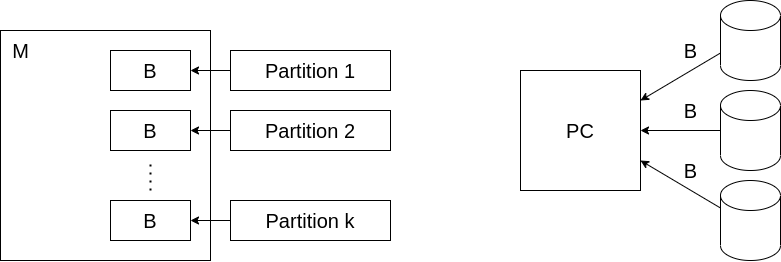
\includegraphics[width=300px]{images/2_Sorting/multi-disks.png}
    \caption{K-way merge-sort with multi-disks}
\end{figure}

If I load concurrently from the 3 disks in 1 I/O I fetch 3 blocks (pages). But that's true only if at each I/O we fetch from different disks!
Merge sort in particular can be fully parallel but it's cursed (check notes for the full explanation).

Let's assume we have $K$ runs and $K$ disks, fully parallelism is not granted! It depends on the values in the pages.
To obtain better performance we can create runs with round robin distribution in disks:
\begin{figure}[H]
    \centering
    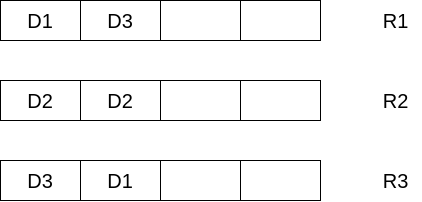
\includegraphics[width=250px]{images/2_Sorting/multi-disks-round-robin.png}
    \caption{round robin distribution of runs in disks}
\end{figure}

What we can do to improve the efficiency without adding too much complexity is called \emph{disk striping} and is already used inside Linux: we assume that all pages at the same time are part of a single large block of size $B \cdot D = B'$.
Programs doesn't see multiple disks, it sees one big disks in which for each I/O we retrieve $B'$ instead of $B$ so our complexity becomes:
$$
    Sort(n, M, B') = O\left( \frac{n}{B'}log_{\frac{M}{B'}} \frac{n}{M} \right) = O \left( \frac{n}{DB}log_{\frac{M}{DB}} \frac{n}{M} \right)
$$

To notice that the more disk i buy (increase $D$), the more runs we need to do, cause the log base is $\frac{M}{DB}$.

How much disk striping outperforms compared with the optimal algorithm, which is $\Theta \left( \frac{n}{DB} log_{\frac{M}{B}} \frac{n}{M} \right)$?
$$
    \frac{ \frac{n}{DB} log_{\frac{M}{DB}} \frac{n}{M} }{ \frac{n}{DB} log_{\frac{M}{B}} \frac{n}{M} } = \frac{ \frac{log_2 \frac{n}{M}}{log_2 \frac{M}{DB}} }{ \frac{log_2 \frac{n}{M}}{log_2 \frac{M}{B}} } = \frac{ log \frac{M}{B} }{ log \frac{M}{DB} } = \frac{ log \frac{M}{B} }{ log \frac{M}{B} - log D } = \frac{1}{1 - log_{ \frac{M}{B} } D}
$$
since we fit $DB$ inside the memory we can say $DB \leq M \implies D \leq \frac{M}{B}$ so we can say:
$$
    \frac{1}{1 - log_{ \frac{M}{B} } D} \geq 1
$$
so there is some outperforming but it's not that much until we get too many disks (eg. for $D=1$ the algorithm is optimal), and moreover it is transparent to the algorithm!

\section{Quicksort}
The quicksort follows the distribution-based pattern. The pseudo-code is:
\begin{verbatim}
    QS(S, i, j)
        if(i < j)
            m = Partition(S, i, j) // m is the position of pivot
            QS(S, i, m)
            QS(S, m+1, j)
\end{verbatim}
the \verb|Partition(S, a, b)| is a procedure which:
\begin{itemize}
    \item chooses a "good" pivot and swaps it with the first element of the partition:
    \begin{figure}[H]
        \centering
        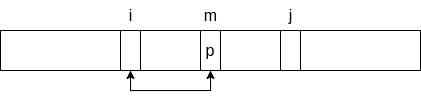
\includegraphics[width=200px]{images/2_Sorting/swap.png}
        \caption{Swap pivot}
    \end{figure}
    
    \item loops over the partition and builds it in the following way:
    \begin{figure}[H]
        \centering
        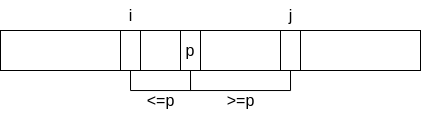
\includegraphics[width=200px]{images/2_Sorting/partitioned.png}
        \caption{Build new partitions}
    \end{figure}
\end{itemize}
We have different strategies to build our partitions:
\begin{itemize}
    \item 1 pivot and 2 partitions;
    \item 1 pivot with 3 partitions:
    \begin{figure}[H]
        \centering
        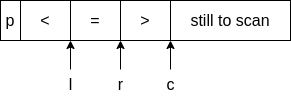
\includegraphics[width=175px]{images/2_Sorting/three-way-partitioning.png}
        \caption{three-way partitioning}
    \end{figure}
    in particular while scanning we can have:
    \begin{itemize}
        \item $S[c] < p$: so we swap $l$ with $c$ and increment $l$;
        \item $S[c] == p$: so we swap $r$ with $c$ and increment both $r$ and $c$;
        \item $S[c] > p$: so we just increment $c$.
    \end{itemize}
    at the end we need to swap $l$ with $pos(p)$ because $p$ is mis-positioned.
    
    \item 3 pivot with 3 partitions: let's assume we have $p'$, $p''$ and $p'''$ and they are $p' < p'' < p'''$ so we use $p''$ as pivot.
\end{itemize}

Let's prove that in case of random choice of pivot we have optimal number of comparison:
$$
    X_{u,v} = 
    \begin{cases}
        1 & \text{iff $S[u]$ cmp $S[v]$} \\
        0
    \end{cases}
$$
we want the average number of comparison so:
$$
    \mathbb{E} \left[ \sum_{u < v} X_{u,v} \right] =  \sum_{u < v} \mathbb{E} \left[ X_{u,v} \right] = \sum_{u < v} 1 \cdot \mathbb{P} \left( S[u] \text{ cmp } S[v] \right) + 0 \cdot \mathbb{P} \left( S[u] \text{ not cmp } S[v] \right)
$$
$$
    = \sum_{u < v} \mathbb{P} \left( S[u] \text{ cmp } S[v] \right)
$$
there is a comparison between $S[u]$ and $S[v]$ only if one of them is chosen as pivot but they can be compared later in recursion too, so the probability depends on the chosen pivot!

$$
    = \sum_{u < v} \mathbb{P} \left( S[u] \text{ is pivot or } S[v] \text{ is pivot} \right)
$$

Let's take the sorted array to reason about the comparisons we can have:
\begin{figure}[H]
    \centering
    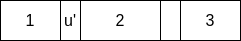
\includegraphics[width=150px]{images/2_Sorting/probability.png}
    \caption{Array zones}
\end{figure}
\begin{itemize}
    \item if pivot is in 1 or 3 there is the probability that $u$ and $v$ will be compared later in recursions;
    \item if pivot is in 2 then recursion will never compare $u'$ and $v'$.
\end{itemize}
So we can have:
\begin{itemize}
    \item $\hat{S}[u']$ is pivot:
    $$
        \frac{1}{v' - u' + 1}
    $$
    
    \item $\hat{S}[v']$ is pivot:
    $$
        \frac{1}{v' - u' + 1}
    $$
    
    \item $\hat{S} < p < \hat{S}[v']$: no comparison
    
    \item $p < \hat{S}[u']$ or $p > \hat{S}[v']$: recursion.
\end{itemize}
So 
$$
    \mathbb{P} \left( S[u] \text{ cmp } S[v] \right) = \frac{2}{v' - u' + 1}
$$
now we can rewrite:
$$
    \sum_{u < v} \mathbb{P} \left( S[u] \text{ is pivot or } S[v] \text{ is pivot} \right) =  \sum_{u < v} \mathbb{P} \left( S[u] \text{ cmp } S[v] \right) = \sum_{u < v} \frac{2}{v' - u' + 1}
$$
$$
    = 2 \sum_{u'=1}^n \sum_{k=2}^{n-u'+1} \frac{1}{k} \leq \sum_{u'=1}^{n} \sum_{k=2}^{n} \frac{1}{k} \leq 2n \cdot \ln n
$$
with the last inequality from the harmonic series.

\subsection{Selection of the k-th ranked element}
Assume we have $S = [2, 7, 6, 3, 8]$ and we want to get the $4^{th}$ ranked element, which is the $k^{th}$ element in sorted array.
We don't want to sort (which would take $O(nlogn)$) so we use the quicksort approach: we select a pivot $m$ whose value is $p$ and we do a single recursion to avoid the whole sorting cost.
We can also exploit the three-way partitions:
\begin{itemize}
    \item if $k$ is in the low half part we recurse on it;
    \item if $k$ is in the high half part we recurse on it;
\end{itemize}
NB: we know the position because $p$ is in it's right place so we can compare $m$ with $k$:
\begin{itemize}
    \item $k < m$: search in lower part for $k$;
    \item $k > m$: search in higher part for $k-m$
\end{itemize}

The complexity of this algorithm is:
$$
    T(n) = O(n) + \mathbb{P}(\text{go to left}) \cdot T(n_<) + \mathbb{P} (\text{go to right}) \cdot T(n_>)
$$
NB: in quick-sort formulation we have no probability since we recurse both on the left and on the right.

Let's restrict to good case: $n_<$ and $n_>$ both $\leq \frac{2}{3}n$, that means:
\begin{itemize}
    \item $n_< \leq \frac{2}{3}n$: pivot is in the first $\frac{2}{3}$ of the array;
    \item $n_> \leq \frac{2}{3}n$: pivot is in the last $\frac{2}{3}$ of the array;
\end{itemize}
so we have pivot in $[\frac{1}{3}n, \frac{2}{3}n]$, and in the end the relation becomes:
$$
    T(n) \leq O(n) + \frac{2}{3} T \left( \frac{2}{3}n \right) + \frac{1}{3}T(n) \implies
$$
$$
    \frac{2}{3}T(n) \leq O(n) + \frac{2}{3} T \left( \frac{2}{3}n \right) \implies
$$
$$
    T(n) \leq \frac{3}{2}O(n) + T \left( \frac{2}{3}n \right) \implies
$$
$$
    T(n) \leq O(n) + T \left( \frac{2}{3}n \right)
$$
and according to Master's Theorem it's $O(n)$.

In terms of I/Os we have $O\left( \frac{n}{B} \right)$.


\subsection{Bounded Quicksort}
We have recursive calls which in the worst case are $n$, in that case we double the occupied space which is very bad.
We can apply the technique known as \emph{removal of tail recursion} rewriting the algorithm in this way:
\begin{verbatim}
    BQS(S, i, j):
        while(j-i > n0){
            r = random pos in {i, _, j}
            swap S[r] and S[i]
            m = Partition(S, i, j)
            if (m <= (i+j)/2){
                BQS(S, i, m-1);
                i = m+1
            }
            else{
                BQS(S, m+1, j);
                j=m-1
            }
        }
        InsertionSort(S i, j) // when array is in cache
\end{verbatim}
in this implementation the number of recursive call is always $O(logn)$:
\begin{figure}[H]
    \centering
    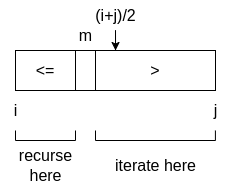
\includegraphics[width=150px]{images/2_Sorting/bqs.png}
    \caption{Bounded quick-sort}
\end{figure}

\subsection{Multi-way Quicksort}
We can build a new version of quicksort with the multi-way approach:
\begin{itemize}
    \item pick $k-1$ different pivots: $S_1$, $S_2$, $\_$, $S_{k-1}$ supposing $S_0 = - \infty$ and $S_k = \infty$.
    It takes $O\left(\frac{n}{B} \right)$;

    \item sort them: $- \infty = S_0 < S_1 < \_ < S_{k-1}  < S_k = \infty$. It takes $O(k logk)$;
    
    \item distribute the array $S$ among the different $S_i$s. We basically scan from left to right and build some blocks such that $B_i = \{ S[j] : S_{i-1} < S[j] \leq S_i  \}$:
    \begin{figure}[H]
        \centering
        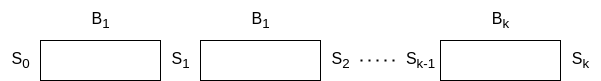
\includegraphics[width=250px]{images/2_Sorting/multiway-partitioning.png}
        \caption{Multi-way partitioning}
    \end{figure}
\end{itemize}
We need to allocate those blocks but how can we know the size to allocate?
We can start to scan $S$ (in $O \left(\frac{n}{B} \right)$), we find the block in which we need to insert the element (in $Ologk$).
We allocate one block $B$ for each of the $B_i$ we are working with, when one block is filled we flush it in memory and fetch another one to fill:

\begin{figure}[H]
    \centering
    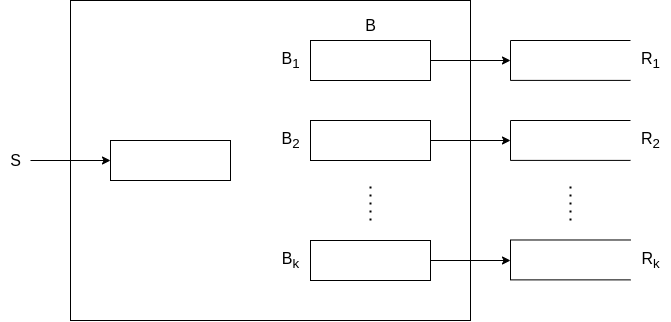
\includegraphics[width=250px]{images/2_Sorting/multiway-partitioning-practice.png}
    \caption{Multi-way partitioning in practice}
\end{figure}
And then we go recursively for each $B_i$: instead of binary way we go $k$-way.
We can have at most $k = \Theta \left( \frac{M}{B} \right)$ so we have $O\left( log_k \frac{n}{B} \right) = O\left( log_{\frac{M}{B}} \frac{n}{B} \right)$ recursive calls and each of them is $O\left( \frac{n}{B} \right)$ since we do a complete scan of the array.
That's true in the average case!

We would like to have balanced partitions with $\frac{n}{k}$ elements in each partition so we can't take $k$ pivots randomly, it would not work for our case. We can do \emph{oversampling}: we pick $(a+1) \cdot k - 1$ samples at random from $S$, we sort them, we pick as pivots $S_i = Sorted[(a+1) \cdot i]$ with $i = 1, 2, \_, k-1$. 
So we pick as pivots elements with at least $(k+1)$ distance from one another.

Let's prove that buckets are always good: let's estimate the probability that one of the bucket is bad:
$$
    \mathbb{P} \left( \exists B_i : |B_i| \geq \frac{4n}{k} \right)
$$
considering $S_{sorted}$:
\begin{figure}[H]
    \centering
    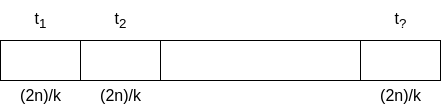
\includegraphics[width=200px]{images/2_Sorting/s_sorted.png}
    \caption{$S_{sorted}$}
\end{figure}
we have as much as $\frac{n}{ \frac{2n}{k} } = \frac{k}{2}$ blocks.
$|B_i| \geq \frac{4n}{k}$ means that a logical block ($t_i)$ is totally included so: $S_{i-1} < B_i \leq S_{i}$:
\begin{figure}[H]
    \centering
    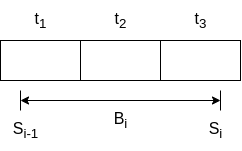
\includegraphics[width=150px]{images/2_Sorting/included_block.png}
    \caption{$t_2$ is fully included in $B_i$}
\end{figure}
but in $B_i$ there are at least $a$ elements, the sorted samples, so:
$$
    \mathbb{P} \left( \exists B_i : |B_i| \geq \frac{4n}{k} \right) \leq \mathbb{P} (\exists t_j : t_j \text{ contains } < a+1 \text{ samples })
$$
$$
    \leq \frac{k}{2} \cdot \mathbb{P} (\text{specific } t_j : t_j \text{ contains } < a+1 \text{ samples })
$$

Now we need to estimate the average number of samples inside a block:
\begin{itemize}
    \item the probability for an item to appear inside a block (let's say $t_2$) is:
    $$
        \mathbb{P}(\text{sample occurs in }t_2) = \frac{ \frac{2n}{k} }{n} = \frac{2}{k}
    $$
    
    \item let's say $X = \#$samples in $t_2$ and:
    $$
    X_i = 
    \begin{cases}
      1 & \text{if $S[i]$ falls in $t_2$} \\
      0 & \text{otherwise}
    \end{cases}
    $$
    then $X = \sum_{i=1}^n X_i$. Now we can calculate the average number of samples inside a block:
    $$
        \mathbb{E}[X] = \sum_{i=1}^{A} \mathbb{E}[X_i] = \sum_{i=1}^{A} 1 \cdot \frac{2}{k} = \frac{2}{k} A
    $$
    with $A=(a+1)k - 1$ as the number of samples.
\end{itemize}
Now we can estimate:
$$
    \mathbb{P} (t_2 \text{ contains } < a+1 \text{ samples }) = \frac{2}{k}A = \frac{2}{k}\left[ (a+1)k -1 \right] = 2(a+1) - \frac{2}{k} 
$$
knowing that $k \geq 2$ we say that $\frac{2}{k} \leq 1$ so:
$$
    \mathbb{P} (t_2 \text{ contains } < a+1 \text{ samples }) \geq 2(a+1)-1 \geq \frac{3}{2}(a+1)
$$
Again:
$$
    \mathbb{E}[X]=\frac{2}{k}A = \frac{2}{k}[(a+1)k - 1] \geq \frac{3}{2}(a+1) \implies
$$
$$
    \frac{2}{3}\mathbb{E}[X] \geq (a+1) \implies
$$
$$
    \left(1-\frac{1}{3}\right)\mathbb{E}[X] \geq (a+1)
$$

So using the previous result we can upper bound:
$$
    \mathbb{P} (t_2 \text{ contains } < a+1 \text{ samples }) = \mathbb{P}\left(X < (a+1)\right) \leq \mathbb{P}\left(X < \left(1-\frac{1}{3}\right) \mathbb{E}[X] \right)
$$
What is the probability of having a value which is strictly less than a factor of the average?
We can use the \emph{Chernoff's bound}:
$$
    \mathbb{P}(X < (1- \delta)\mathbb{E}[X] ) \leq e^{\frac{-\delta^2}{2}\mathbb{E}[X]}
$$
applying that bound we reach:
$$
    \mathbb{P} (t_2 \text{ contains } < a+1 \text{ samples }) \leq e^{-\frac{1}{18}\mathbb{E}[X]} \leq e^{-\frac{1}{18} \cdot \frac{3}{2}(a+1)} = e^{-\frac{a+1}{12}}
$$

In the end we have:
$$
    \frac{k}{2} \cdot \mathbb{P} (t_2 \text{ contains } < a+1 \text{ samples }) \leq \frac{k}{2} \cdot e^{-\frac{a+1}{12}} = \frac{k}{2} e^{-\frac{12ln(k)}{12}} = \frac{k}{2}e^{-ln(k)} = \frac{k}{2k}
$$
$$
    = \frac{1}{2}
$$
The probability of having a wrong partitioning is less than $\frac{1}{2}$ so we oversample, we build the buckets, if we are in a bad case we re-run the oversample and partition again.

